%%%%%%%%%%%%%%%%%%%%%%%%%%%%%%%%%%%%%%%%%%%%%%%%%%%%
%%%% En-tête leçon
\begin{headerBlock}
  \chapter{Phénomènes de résonance dans différents domaines de la physique}
  \label{LP_resonance} 
\end{headerBlock}

%%%%%%%%%%%%%%%%%%%%%%%%%%%%%%%%%%%%%%%%%%%%%%%%%%%%
%%%% Références
\begin{center}
\begin{tabularx}{\textwidth}{| X | X | c | c |}
  \hline
  \rowcolor{gray!20}\multicolumn{4}{c}{Bibliographie de la leçon : } \\
  \hline 
  Titre & Auteurs & Editeur (année) & ISBN \\
  \hline
  Mécanique & J.M Brébec & HPrépa & \\
  \hline 
  & & &    \\
  \hline 
  & & &    \\
  \hline 
\end{tabularx}
\end{center}

%%%%%%%%%%%%%%%%%%%%%%%%%%%%%%%%%%%%%%%%%%%%%%%%%%%%
\begin{reportBlock}{Commentaires des années précédentes :}
    \begin{itemize}
        \item \textbf{2015 :}Présenter l’exemple célèbre du pont de Tacoma n’est pas pertinent, sauf s’il s’agit d’effectuer une critique d’une interprétation erronée très répandue,
        \item \textbf{2010 :} L’analyse du seul circuit RLC est très insuffisante pour cette leçon. Le phénomène de résonance ne se limite pas aux oscillateurs à un degré de liberté.
    \end{itemize}
\end{reportBlock}
%%%%%%%%%%%%%%%%%%%%%%%%%%%%%%%%%%%%%%%%%%%%%%%%%%%%
%%%% Plan
\begin{reportBlock}{Plan détaillé}

  \textbf{Niveau choisi pour la leçon :} Licence 3
  \newline
  \textbf{Prérequis} : \begin{itemize}
      \item Mécanique newtonienne
      \item Optique ondulatoire
      \item Electrocinétique
  \end{itemize}

  \textbf{Déroulé détaillé de la leçon: }  
  
\section*{Introduction}
Définition : pour un système auquel qu'on soumet à une excitation sinusoïdale de pulsation $\omega$, la réponse du système est maximale à la pulsation $\omega_r$, appelée fréquence de résonance.

\section{Oscillateurs harmoniques forcés}

\subsection{Résonance en vitesse en régime forcé} 

\textcolor{red}{Attention, faire la discussion sur la phase}. Interprétation énergétique possible.

\subsection{Equivalent électrocinétique}
Démontrer la résonance en tension de la capacité d'un circuit RLC série.\\

Déterminer la fréquence de résonance et comparer avec les valeurs obtenues pour le RLC-mètre. On peut aussi observer l'évolution de la résonance à le changement de la résistance, le relié au facteur de qualité.

\section{Oscillateurs couplés}
Interprétation en terme d'excitation de mode propre.
\begin{center}
    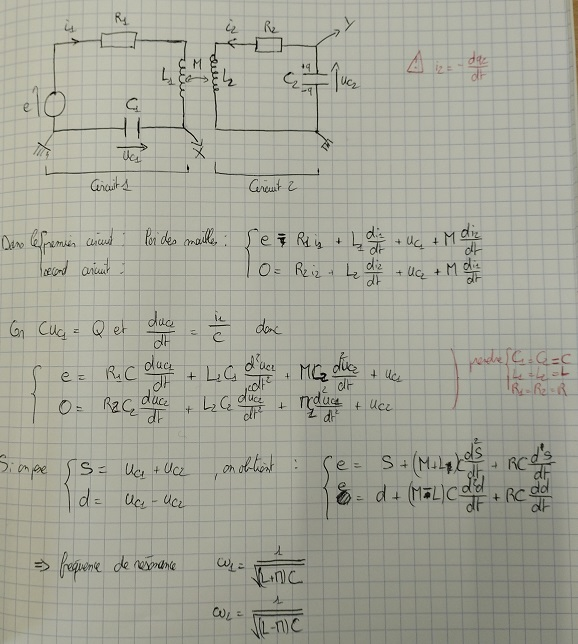
\includegraphics[scale=0.5]{LP_Resonance/Oscillateurs_couple.jpg}
\end{center}    


\textcolor{blue}{Expérience : }montrer l'influence du couplage sur la résonance du premier circuit RLC à l'aide d'un deuxième circuit RLC. Intérêt pratique ?

\section{Cavité résonante}
\subsection{Cavité Fabry Pérot}
\subsection{Intensité transmise}
Calcul possiblement à faire soit hyper rapidement, soit en prérequiss.

\subsection{Finesse}
\end{reportBlock}